\subsubsection{Basic recurrent model}

This model is the same as the dense model but with the addition of a new simple recurrent layer explained in section \ref{rnn_theory}. The simple recurrent layer is a layer that allows us to use information from other previous intervals that will be used for the final prediction. This recurrent layer has $100$ units and graphically the model can be represented as follows:

\begin{figure}[H]
    \centering
    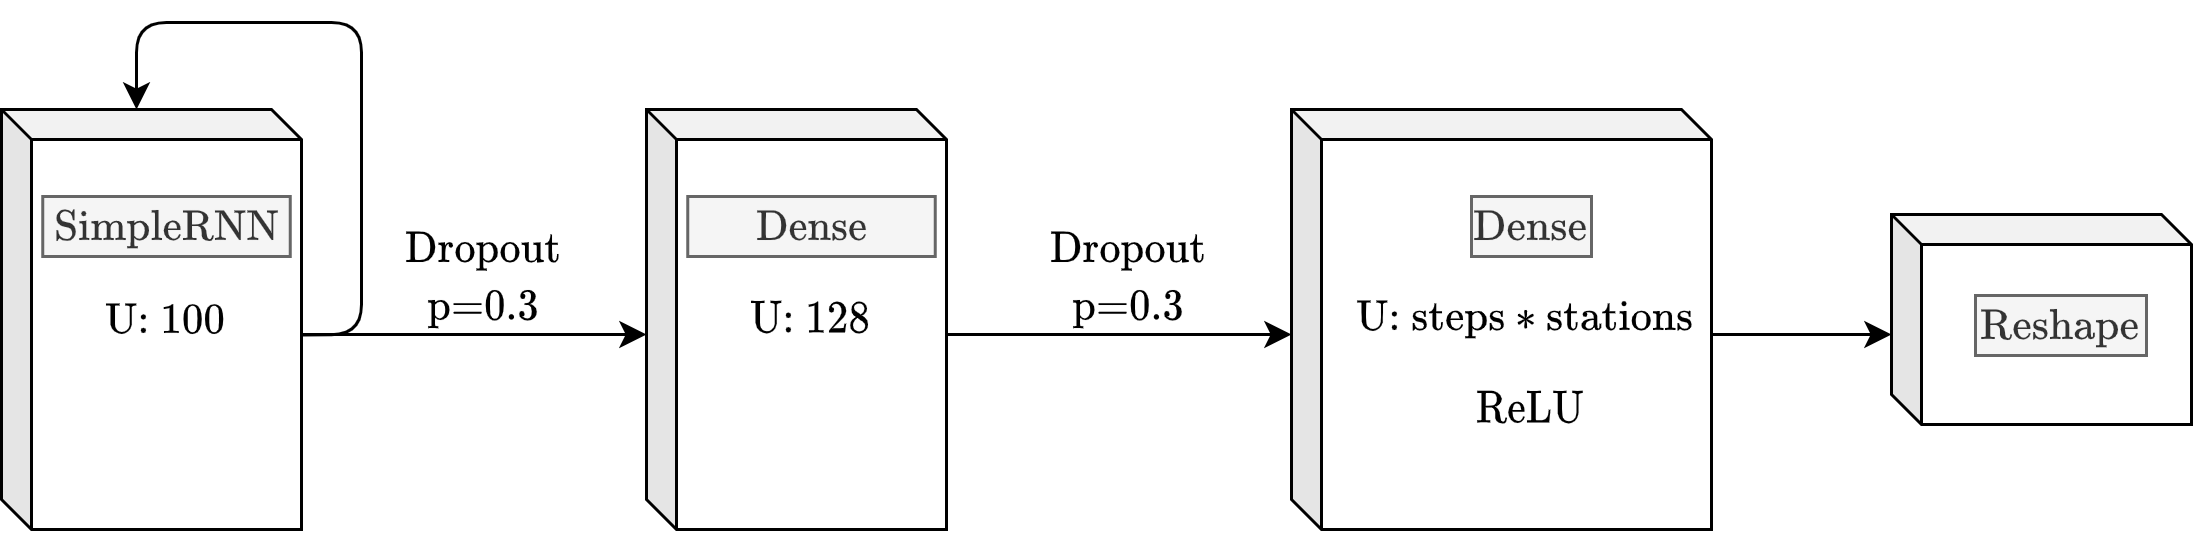
\includegraphics[width=12cm]{images/solution/models/simpleRnn.png}
    \caption{Basic recurrent model}
    \label{fig:dense-model}
\end{figure}

As you can see it is an extension of the dense model explained in the previous section but adding a new \textit{SimpleRNN} type layer. The code of this model has been defined as shown below:

\begin{minted}[fontsize=\scriptsize]{python}
from tensorflow.keras.models import Sequential
from tensorflow.keras.layers import Reshape, Dense, Dropout, Lambda, SimpleRNN

# `steps` is a variable which has the number of intervals to be predict
steps = 0 

# `stations` is the number of stations in the bike network
stations = 0

rnn_model = Sequential([
    # RNN layer
    SimpleRNN(100, return_sequences=True),
    
    Dropout(0.3),
    Dense(128),
    Dropout(0.3),
    
    # Ouput layer
    Dense(steps * stations),
    
    # Vector to matrix
    Reshape([steps, stations])
])
\end{minted}

The results of the model can be seen together with the other results in section \ref{results}.